\section{Our Approach}
\label{sec:approach}

In this section, we first define the proposed {\em association
network}, then show how to populate such network. We then
propose algorithms to compute relatedness using this network,
and finally conclude with some discussions. 

\subsection{Association network}
\label{sec:definition}

%Let $T$ denote a set of terms $t$ and $C$ denote a set of Wikipedia concepts
%(or articles) $c$.
A {\em super node} $s$ represents a set of synonymous terms
%\footnote{Here by ``related'' we mean either lexicographically
%similar or semantically very close, as formally defined in Algorithm
%\ref{algo:bootstraping}.} 
and their corresponding Wikipedia concepts (or article pages), 
denoted as $(T, C)$, where $T$
is a set of terms and $C$ is a set of Wikipedia concepts. For
example, $(\{apple, apples\}, \{Apple, Apple\ Inc.\})$ is one such
super node. Given a term $t$, we can generate a super node $s$ by
Algorithm \ref{algo:bootstraping}.
%Similarly a concept can also be mapped to a unique $s$.
$def_c(t)$ returns a set of Wikipedia concepts defining $t$, 
while $def_t(c)$ returns a set of terms defined by $c$. 
We say $t$ is defined by $c$ if
$t$, as an anchor text, links to $c$ at least 10\% of the time, and
$c$ is being linked from $t$ at least 10\% of the time. 
We found the results to be insensitive to the value of 10\%, 
which was empirically determined.

\begin{algorithm}[th]
\caption{Generate super node}
\label{algo:bootstraping}
\begin{algorithmic}[1]
\Function{Bootstrap}{term $t$}

\State $T \leftarrow \{t\}, C \leftarrow \{\}$
\While{$T$ or $C$ is updated}
\For{$t \in T$}
\State $C \leftarrow C \cup def_c(t)$
\EndFor
\For{$c \in C$}
\State $T \leftarrow T \cup def_t(c)$
\EndFor
\EndWhile
\State \textbf{return} $(T, C)$

\EndFunction
\end{algorithmic}
\end{algorithm}

Our association network is a weighted directed graph $G (V, E)$,
with $w(e)$ denoting the weight of edge $e$ ($e\in E$). Each vertex
in the graph is a super node $s$, and an edge $e(u, v)$ 
($u, v\in V$) indicates $u$ can associate to $v$, with strength $w(e)$.
%quantifying the strength. 
%To comply with the conventional definition of association strength
%established in free association research, 
For all $u\in V$, strength is normalized:
%the following equation is required to hold true.
\begin{equation}
\sum_{v} w(u, v) = 1
\label{eq:normalize}
\end{equation}
%
%Note, we define each vertex to be a super node, which may include
%unambiguated concepts of a term (e.g. Apple and Apple Inc.). The
%reasons for this will be discussed in \secref{sec:discussion}.

\subsection{Network construction}
\label{sec:construction}

%We then propose to populate the association network from Wikipedia,
%which we define as  \emph{network construction problem}, formally as:
Given a set of terms $T_0$, we populate an association network $G
(V, E)$ in two steps:
%such that every vertex $v$ is a super node generated from $t$ ($t\in T$),
%and for all $t\in T$, $t$ is contained in exactly one $v$.
first determine the vertex set $V$ in our network, and then determine edge set
$E$ and estimate the association
strengthes for edges in the network. 
%To estimate the strengths,
%we integrate several types of co-occurrence information to
%compute a single, universal strength score.
%therefore some discussion about the co-occurrence information we use
%and how we integrate them will also be included.

To determine the vertex set $V$ of our association network $G$, we
run Algorithm \ref{algo:bootstraping} for every $t\in T_0$, such
that the set of all output super nodes is $V$. Algorithm
\ref{algo:bootstraping} ensures $V$ to have the following property
\footnote{The proof of this lemma is given at
\url{http://adapt.seiee.sjtu.edu.cn/~keyang/assoc/}.}:

\begin{lemma}
Each term $t$ in $T_0$ appears in exactly one vertex of $G$, and
no two vertices share an identical concept $c$.
\end{lemma}

To determine the edge set $E$ of our association network and the
association strength of each $e \in E$, we tap into five types of
co-occurrences in Wikipedia to compute five association strength scores, which are then integrated by a
linear weighted sum, where the weight parameters are trained 
using free association norms labeled by human beings. 
%Next, we will state clearly the five types of co-occurrence that we use, 
%and then explain how we integrate them into a single strength score.

These five types of co-occurrences are sentence level co-occurrences
({\em slc}), title link co-occurrences ({\em tlc}), title gloss
co-occurrences ({\em tgc}), title body co-occurrences ({\em tbc}), and
category level co-occurrences ({\em clc}). Examples of these
co-occurrences are shown in \figref{fig:cooccur}.

\begin{figure}[htb]
\centering
\epsfig{file=figure/cooccur_small.eps, width=1\columnwidth}
\caption{Five types of co-occurrences in Wikipedia}
\label{fig:cooccur}
\end{figure}

Specifically, {\em slc} refers to the co-occurrence of two terms in one
sentence, such as {\em water} and {\em precipitation}. 
{\em tlc} refers to the co-occurrence of the page's title and
anchor text in the page, such as {\em river} and {\em lake}, {\em
river} and {\em precipitation}. {\em tgc} refers to the co-occurrence of a
page's title and an unlinked term in the \emph{gloss}, or the
definition paragraph of this page, such as {\em river} and {\em
stream}. {\em tbc} refers to the co-occurrence of a page's title and an
unlinked term in the body paragraphs, the paragraphs except
for gloss, such as {\em river} and
{\em water}. {\em clc} refers to the number of categories in which
two concepts co-occur, 
e.g., the concepts {\em Lake} and {\em Stream} share the category 
``Bodies of water''.
As described above, slc is between two terms, clc between two concepts,
and the other three between a concept and a term. For all these types
of co-occurrences, we first map the term or the concept
to the corresponding super node, and then count the frequency.

%tlc, tgc and tbc
%capture the co-occurrence between a particular concept and the term
%explaining or describing this concept. We treat them as
%alternative sources of co-occurrence to reflect the intuition that
%the linked terms and the terms in gloss are usually more important
%to the title than other terms. clc is particularly good at capturing
%the co-occurrence of two concepts within a type hierarchy.

For each type of co-occurrences denoted as $\tau$, where $\tau\in \{slc,
tlc, tgc, tbc, clc\}$, we model the association strength from $u$ to
$v$ after the measure proposed in \cite{Wettler:1993}
%, which in
%their work was used to compute word association based on
%co-occurrence in large corpus. The measure is shown 
in \eqref{eq:cooccur}. Here, $\alpha$ is an exponent
parameter between 0 and 1. $p_\tau(u)$, $p_\tau(v)$ and $p_\tau(u,v)$ is
computed as $\frac{f_\tau(u)}{N_\tau}$, $\frac{f_\tau(v)}{N_\tau}$ and
$\frac{f_\tau(u,v)}{N_\tau}$ respectively, where $f_\tau(u)$, $f_\tau(v)$ is the
occurrence frequencies of $u$, $v$, $f_\tau(u,v)$ is the co-occurrence
frequencies of $u$ and $v$, and $N_\tau$ is the total number of tokens
for a particular $\tau$. We defer the discussion of the choice of $\alpha$ 
till \secref{sec:discussion}.

\begin{equation}
r_\tau(u,v) = \frac{p_\tau(u,v)}{p_\tau(v)^\alpha p_\tau(u)}
\label{eq:cooccur}
\end{equation}

%Then for all $u\in V$, normalization as shown in
%\eqref{eq:normalize2} is conducted to meet the constraint specified
%in \eqref{eq:normalize}.
$r_\tau(u, v)$ is normalized to $w_\tau(u, v)$:
\begin{equation}
w_\tau(u, v) = \frac {r_\tau(u,v)} {\sum_{v}r_\tau(u,v)}
\label{eq:normalize2}
\end{equation}

%\figref{fig:distribution} illustrates the distributions of five
%co-occurrence types on 5 pairs of super nodes.
We perform a case study to examine the different capabilities of
capturing associated pairs by the five types of co-occurrences.
We compare the normalized association strength $w_\tau(u, v)$ for 
every $\tau$ and the result is shown in \figref{fig:distribution}. 
$u$ is set to be the super node of {\em river}, 
and $v$'s are the super nodes of 5 terms most associated with {\em river},
as shown in \tabref{tab:florida}.
%For all co-occurrence
%type $c$, $w_\tau(u, v)$ is computed and normalized to the same scale
%for comparison, where $u$ is the super node generated from the term
%{\em river}, and $v$ is the super node generated from each term
%shown in the X axis, e.g. {\em lake}. 
We observe the following:
i) $slc$ is distributed more uniformly
among the pairs than others ii) only river-lake and river-stream
have $clc$, as lake and stream are in the same type hierarchy as
river iii) $tlc$, $tgc$ and $tbc$ capture the terms explaining or
describing river, basically all the terms except for boat in this
case. This shows that even though slc has been widely used in 
the literature, reflecting related terms of locality, 
other types of co-occurrences, though less studied, 
have complementary strength in terms of capturing associated pairs.

\begin{figure}[htb]
\centering
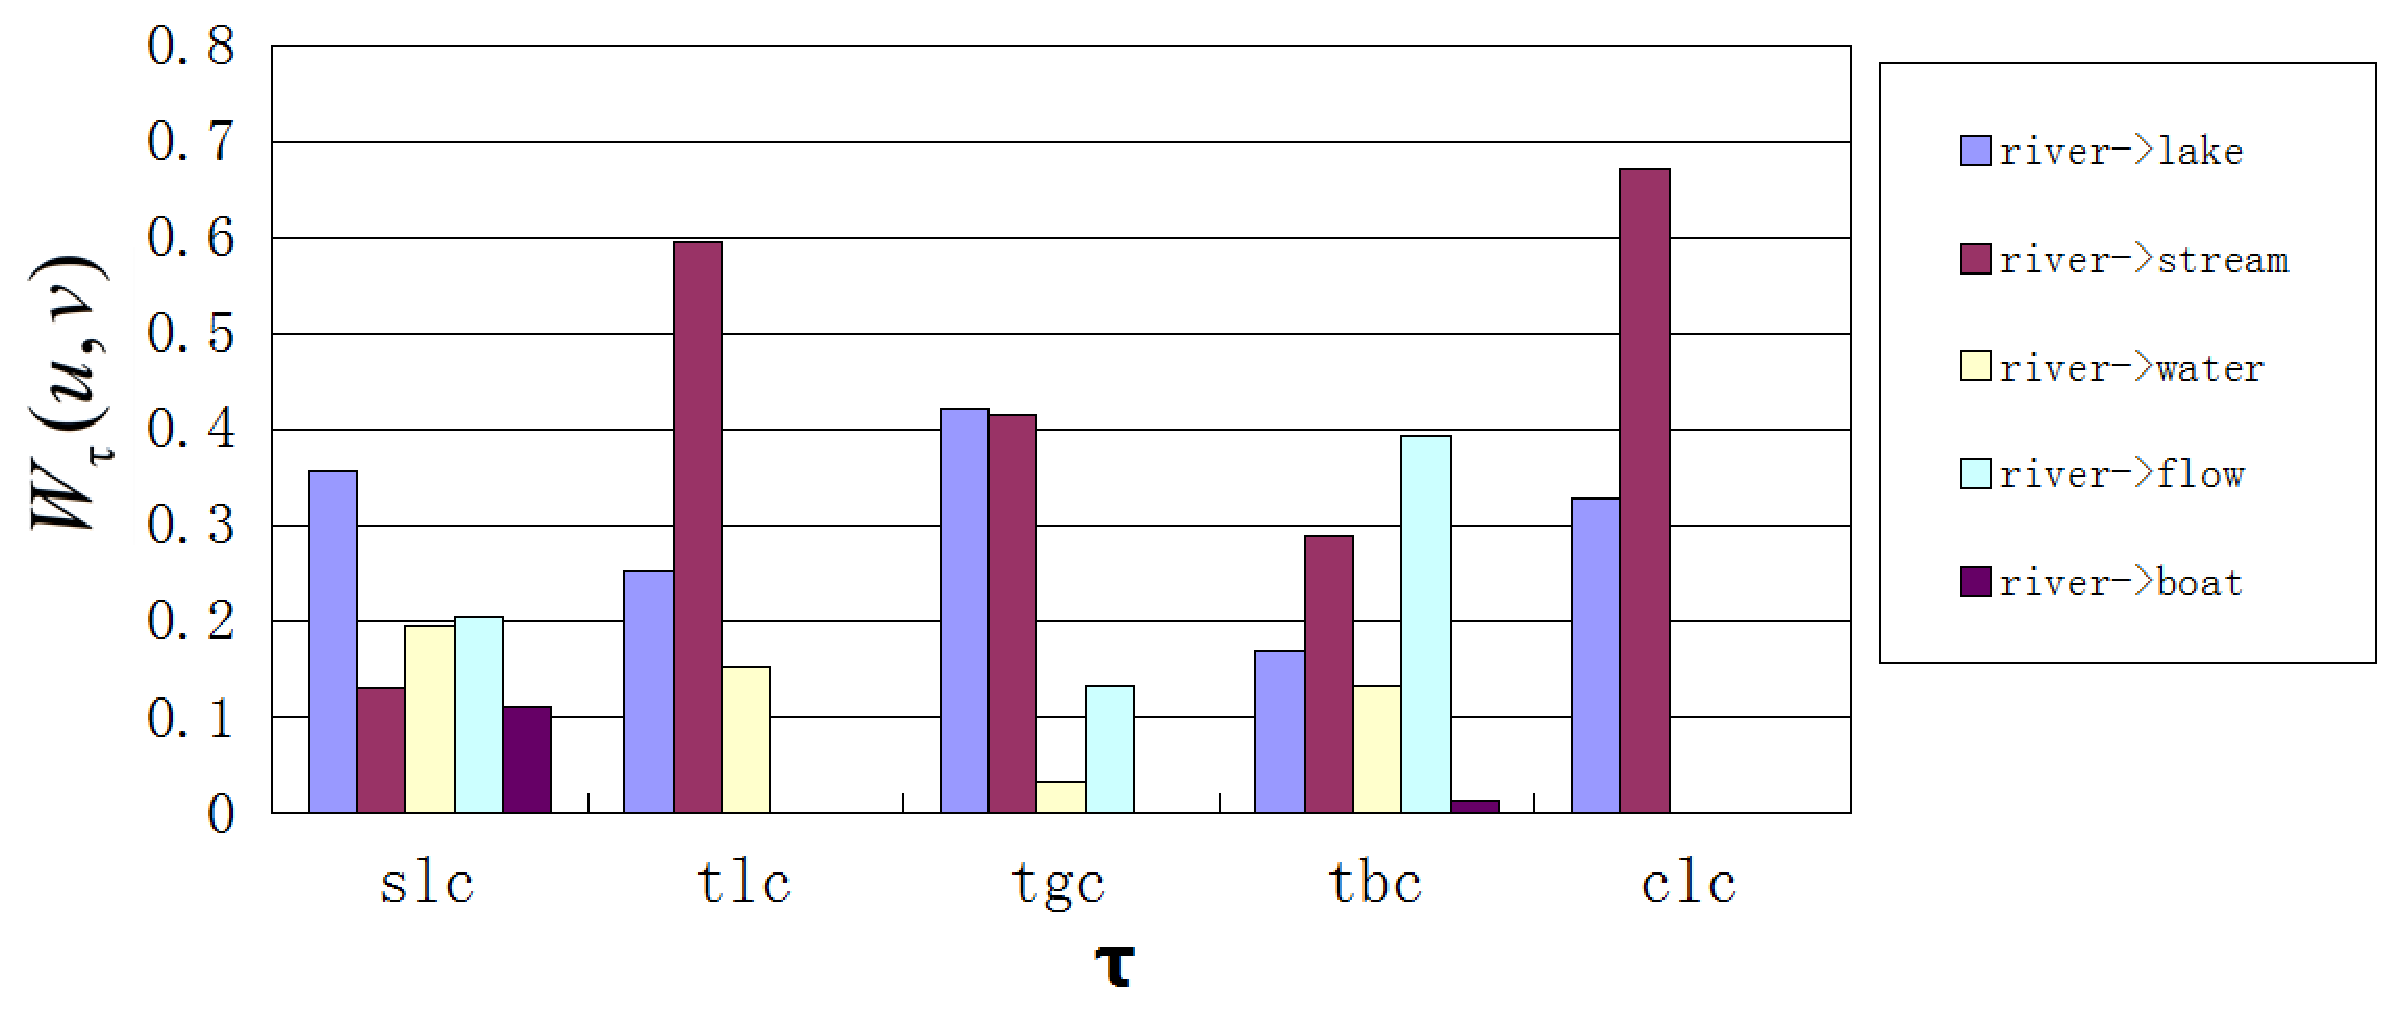
\epsfig{file=figure/distribution.eps, width=\columnwidth}
\caption{Comparison of $w_\tau(u, v)$ for different $\tau$}
\label{fig:distribution}
\end{figure}

We then integrate the five types of $w_\tau(u, v)$ into a single
strength score: $w(u, v) = \sum_{\tau}\theta_\tau w_\tau(u, v)$. 
%as shown in \eqref{eq:integrate}. 
We mimic human perception of relatedness in
determining how to aggregate co-occurrences. Specifically, we train
the weights $\theta_\tau$ through a linear regression on
the Florida Norms.
%Florida norms is the largest free association
%database collected in the United States, in which more than 6,000
%participants produced nearly three quarters of a million responses
%to 5,019 stimulus words.
%%In the experiment collecting the dataset,
%%participants were asked to write down the first word (generally
%%referred as {\em target}) that came to mind that was meaningfully
%%related or strongly associated to the presented word (generally
%%referred as {\em cue}).
%The researchers then computed the
%association strength as a proportion of subjects producing  a
%particular response for the given cue word, to infer the probability
%of producing a particular target in the presence of a given cue
%word.
%For example, for the word ``ability'', 17 out of the 143
%participants in the group produced ``capability'' as a response, so
%the probability of producing ``capability'' in the presence of
%``ability'' is calculated to be 0.119.

We first use the terms appearing in Florida Norms as $T_0$ to 
determine the super node set $V$. 
Then we use every cue-response pair in Florida Norms as a training
instance, with the label being the association strength computed 
form the norms.  For every training instance we
map the two terms into their corresponding super nodes $u$ and $v$, and
calculate $w_\tau(u, v)$ for every $\tau$ as its features. When
performing linear regression, we impose the constraints that
$\sum_{\tau}\theta_\tau = 1$, $0< \theta_\tau < 1$ for all $\theta_\tau$, and
that the intercept term must be equal to 0. The
parameters $\theta_\tau$ are then used to combine the different $w_\tau(u, v)$
regardless of the given $T_0$: As $\sum_{\tau}\theta_\tau = 1$ holds true, it is
easy to attest that the combined strength score $w(u, v)$ meets
the requirement of \eqref{eq:normalize}. An edge $e(u, v)$ exists
if and only if $w(u, v)>0$.

%\begin{equation}
%\begin{aligned}
%& w(u, v) = \sum_{\tau}\theta_\tau w_\tau(u, v)\\
%& s.t. \sum_{\tau}\theta_\tau = 1
%\end{aligned}
%\label{eq:integrate}
%\end{equation}

\subsection{Relatedness computation}
\label{sec:relatedness}

We now present how to leverage the constructed network for computing
relatedness between terms and between short texts.  In both algorithms,
the intention is to leverage the latent {\em bridge} 
vertices between two observed vertices to provide supportive information 
in relatedness computation.
The weight of a bridge vertex, with respect to an unordered pair of 
vertices $\{u, v\}$, is defined as in \eqref{eq:bridge}.
% A vertex is called to be bridge of $\{u, v\}$ if and only if $weight_{\{u, v\}}(x)>0$.

\begin{equation}
W_{\{u,v\}}(x) = \max(w(u,x)\times w(x,v), w(v,x)\times w(x,u))
\label{eq:bridge}
\end{equation}

% \begin{algorithm}[th]
% \caption{Find bridge vertices}
% \label{algo:bridge}
% \begin{algorithmic}[1]
% \Function{FindBridges}{network $G(V, E)$, an unordered pair of vertices $\{u, v\}$}
% \State $X \leftarrow \{\}$
% \For{$x \in V$}
% \If {$weight(x)>0$}
% \State $X \leftarrow X \cup \{x\}$
% \EndIf
% \EndFor
% \State \textbf{return} $X$
% \EndFunction
% \end{algorithmic}
% \end{algorithm}

For term relatedness computation, we first map any given term $t$ to
its corresponding vertex $u$ in the association network. 
The relatedness between any vertex $u$ and itself is always defined to be 1:
$relate(u,u)=1$.
To compute relatedness between two vertices $u$ and $v$, 
our baseline algorithm is to add up the weights of the edges
between $u$ and $v$: 
\begin{equation}
relate(u,v)=w(u,v)+w(v,u)
\label{eq:baseline}
\end{equation} 
This algorithm captures the intuition that if $u$ associates more 
strongly to $v$ or
vice versa, $u$ and $v$ are often more related (see \tabref{tab:florida}).
As validated later in \secref{sec:eval}, despite its usefulness and 
intuitiveness in detecting related pairs, this algorithm leverages
insufficient signals from the association network and hence obtains 
sub-optimal accuracy, especially when the association network is sparse.
Thus, we propose a revised algorithm as a natural extension to the 
baseline: 
\begin{equation}
relate(u,v)=w(u,v)+w(v,u)+\sum_{x\in V}W_{\{u, v\}}(x)
\label{eq:revised}
\end{equation}
% where $X$ is returned by running Algorithm \ref{algo:bridge} using $\{u, v\}$ as input.
This algorithm captures the intuition that if $u$ associates more strongly to $v$, 
directly or indirectly (via some bridge vertices), or vice versa, $u$ and $v$ are often more related.


% For term relatedness, we map any given term $t$ to
% its corresponding vertex $u$ in the association network, then
% represent it by three feature vectors. The first vector, denoted as
% $u_{to}$, is constructed by taking all the vertices that $u$ may
% associate \emph{to} as dimensions, and the corresponding association
% strength as weight in each dimension. The second vector, denoted as
% $u_{from}$, is constructed similarly, except that each dimension is
% the vertex that $u$ may associate \emph{from}. The third vector, denoted as
% $u_{self}$ just has one dimension which is $u$ itself, and the
% weight is defined to be 1.
% For example, when river is associated to canyon, its strength is reflected in
% the vectors of
% ${river}_{to}$ and 
% ${canyon}_{from}$.


%To illustrate, we show here the 10 highest weighted dimensions for
%each of the following 4 vectors: ${river}_{to}$, ${river}_{from}$,
%${lake}_{to}$ and ${lake}_{from}$. As each dimension is a super node,
%we just show here the $t_{init}$ of each super node for illustration.
%
%\begin{itemize}
%\item ${river}_{to}$: canyon, stream, flood, canal, waterfall, valley, lake, dam, creek, swamp
%\item ${river}_{from}$: creek, canyon, waterfall, downstream, upstream, flood, stream, dam, canal, fork
%\item ${lake}_{to}$: pond, salt, river, shore, stream, marsh, swamp, dam, water, trout
%\item ${lake}_{from}$: pond, seepage, salt, outlet, shore, thaw, trout, swamp, dam, marsh
%\end{itemize}
%
% When computing relatedness between two terms, we map them to
% corresponding vertices $u$ and $v$ and compute the three feature
% vectors mentioned above for each. Then, for the total 9 ($3\times3$)
% pairs of vectors, we compute the cosine similarity between
% them to examine if vector directions are similar,
% and then take the average.

% We argue that all of these 9 pairs of vectors are useful signals
% in computing term relatedness/similarity. On one hand, the cosine
% similarities between the vectors of the same type (denoted as
% $cos_{same}$, e.g., $cos(u_{to}, v_{to})$) 
% capture the intuition that if the network contexts of $u$ and $v$ are 
% similar, then $u$ and $v$ are related/similar, 
% e.g., $cos(u_{to},
% v_{to})$ and $cos(u_{from}, v_{from})$ capture the intuition that,
% if the vertices $u$ and $v$ associate to/from are similar, 
% then $u$ and $v$ are related/similar. 
% On the other hand, the cosine similarities between the 
% vectors of the different types (denoted as $cos_{cross}$,
% e.g.,  $cos(u_{to}, v_{self})$ or $cos(u_{to}, v_{from})$)
% capture the intuition that if $u$ could easily 
% associate to/from $v$, directly (e.g., $cos(u_{to}, v_{self})$),
% or indirectly (e.g., $cos(u_{to}, v_{from})$), 
% then $u$ and $v$ are related/similar. 
% In \secref{sec:eval}, we will validate that $cos_{same}$ and $cos_{cross}$ 
% capture not only different, but also complementary signals.

For the short text relatedness computation, 
%our intention is not to develop a specialized scheme for this task,
%but to validate the usefulness of the association network even
%with a simple heuristics:
we abstract a given text as a bag of super nodes, i.e., a vector with each
dimension being a super node and weight in that dimension being
the occurrence frequency of the terms mapping to this super node. While
cosine similarity could be directly computed to measure if two text
vectors are similar or not, it suffers from low accuracy as
semantically similar texts do not necessarily share identical or
synonymous terms with each other. 
Therefore, we expand
the original vectors before computing cosine similarity between two
vectors, by adding bridge vertices identified through our
association network as new dimensions. Algorithm \ref{algo:expand}
shows how we convert the original vector $vec_0$ to the expanded
vector $vec_+$, where $K$ is a parameter controlling the extent of 
the expansion (i.e., higher $K$ means more expanded vertices).

\begin{algorithm}[th]
\caption{Expand vector}
\label{algo:expand}
\begin{algorithmic}[1]
\Function{ExpandVector}{network $G(V, E)$, vector $vec_0$, integer $K$}
\State $vec_+ \leftarrow vec_0$
\For{$u,v \in$dimension set of $vec_0$ and $u\ne v$}
\State $V_K$ = top $K$ vertices in $V$ sorted by weights
\For{$x \in V_K$}
\State $vec_+(x) \leftarrow vec_+(x) + 1$
\EndFor
\EndFor
\State \textbf{return} $vec_+$
\EndFunction
\end{algorithmic}
\end{algorithm}


\subsection{Discussion}
\label{sec:discussion}

%In the following, we discuss some implementation issues.
%
Instead of disambiguating the term occurring in a Wikipedia page to
one of its concepts and defining each vertex to be a disambiguated
concept in the association network, we choose to define each vertex
to be a super node, comprising multiple concepts for a term.
That is because, even though it is possible to disambiguate a term
in Wikipedia pages by taking advantage of contextual information,
such a task is more difficult on the free association norms, where
virtually no context is available. Even worse, the two end-to-end
tasks (term and short text relatedness) also
inherently lack context information to perform reliable
disambiguation.

%There are also other types of co-occurrence in Wikipedia, such as
%{\em co-citation} used in \cite{Adafre:2005}. But we found through
%our preliminary experiments that they are less useful in
%constructing desired association network.
%
When computing the association strength between two super nodes $u$ and
$v$, the parameter $\alpha$ needs to be chosen to instantiate the
general form shown in \eqref{eq:cooccur}. One natural choice is to
set $\alpha$ to be 0, which turns the formula into conditional
probability, i.e., the probability of observing $v$, given $u$.
However, it is argued previously \cite{Wettler:1993,asso09} that 
the conditional probability measure does not take into consideration the
general frequency of the response word and therefore tends to bias
toward highly frequent words, such as function words. As a result, 
we follow \cite{Wettler:1993} to set $\alpha$ to be 0.66, 
which, according to them, perform the best in estimating word association. 
%In all of our experiments, this setting will remain stationary.

Our algorithms for relatedness computation are for showcasing the power of 
the association network, and thus many other algorithms
can be developed to  take advantage of the full potential of the association network.
